\documentclass{article}
\usepackage[margin=2cm]{geometry}
\usepackage[utf8]{inputenc}
\usepackage{minted}
\usepackage{amsfonts}
\usepackage{amsmath}
\usepackage{tikz}
\usepackage{}

\title{CSC258 PRELAB 7}
\author{Tingfeng Xia}
\date{\today}

\usepackage{natbib}
\usepackage{graphicx}

\begin{document}

\maketitle
\section*{PART I}
\paragraph{(9)} I should first present my test cases, below is the writing that we will do. We will read from positions \texttt{00000}, \texttt{01000},\texttt{10000}, and \texttt{11100}. The first three are the three boxes to the top left of the memory block above, while the last one \texttt{11100} is 28 in binary, corresponding to the bottom right box.
\begin{center}
    \begin{tabular}{ ||cccc|cccc|| }
        \hline\hline
        0 & 0 & 0 & 1 & 0 & 0 & 0 & 0 \\ \hline
        0 & 0 & 1 & 0 & 0 & 0 & 0 & 0 \\ \hline
        0 & 0 & 1 & 1 & 0 & 0 & 0 & 0 \\ \hline
        0 & 1 & 0 & 0 & 0 & 0 & 0 & 0 \\
        \hline\hline
    \end{tabular}
\end{center}
Indeed, we have the following in the ModelSim results for the \texttt{ram32x4.v} module that we just created.
\begin{center}
    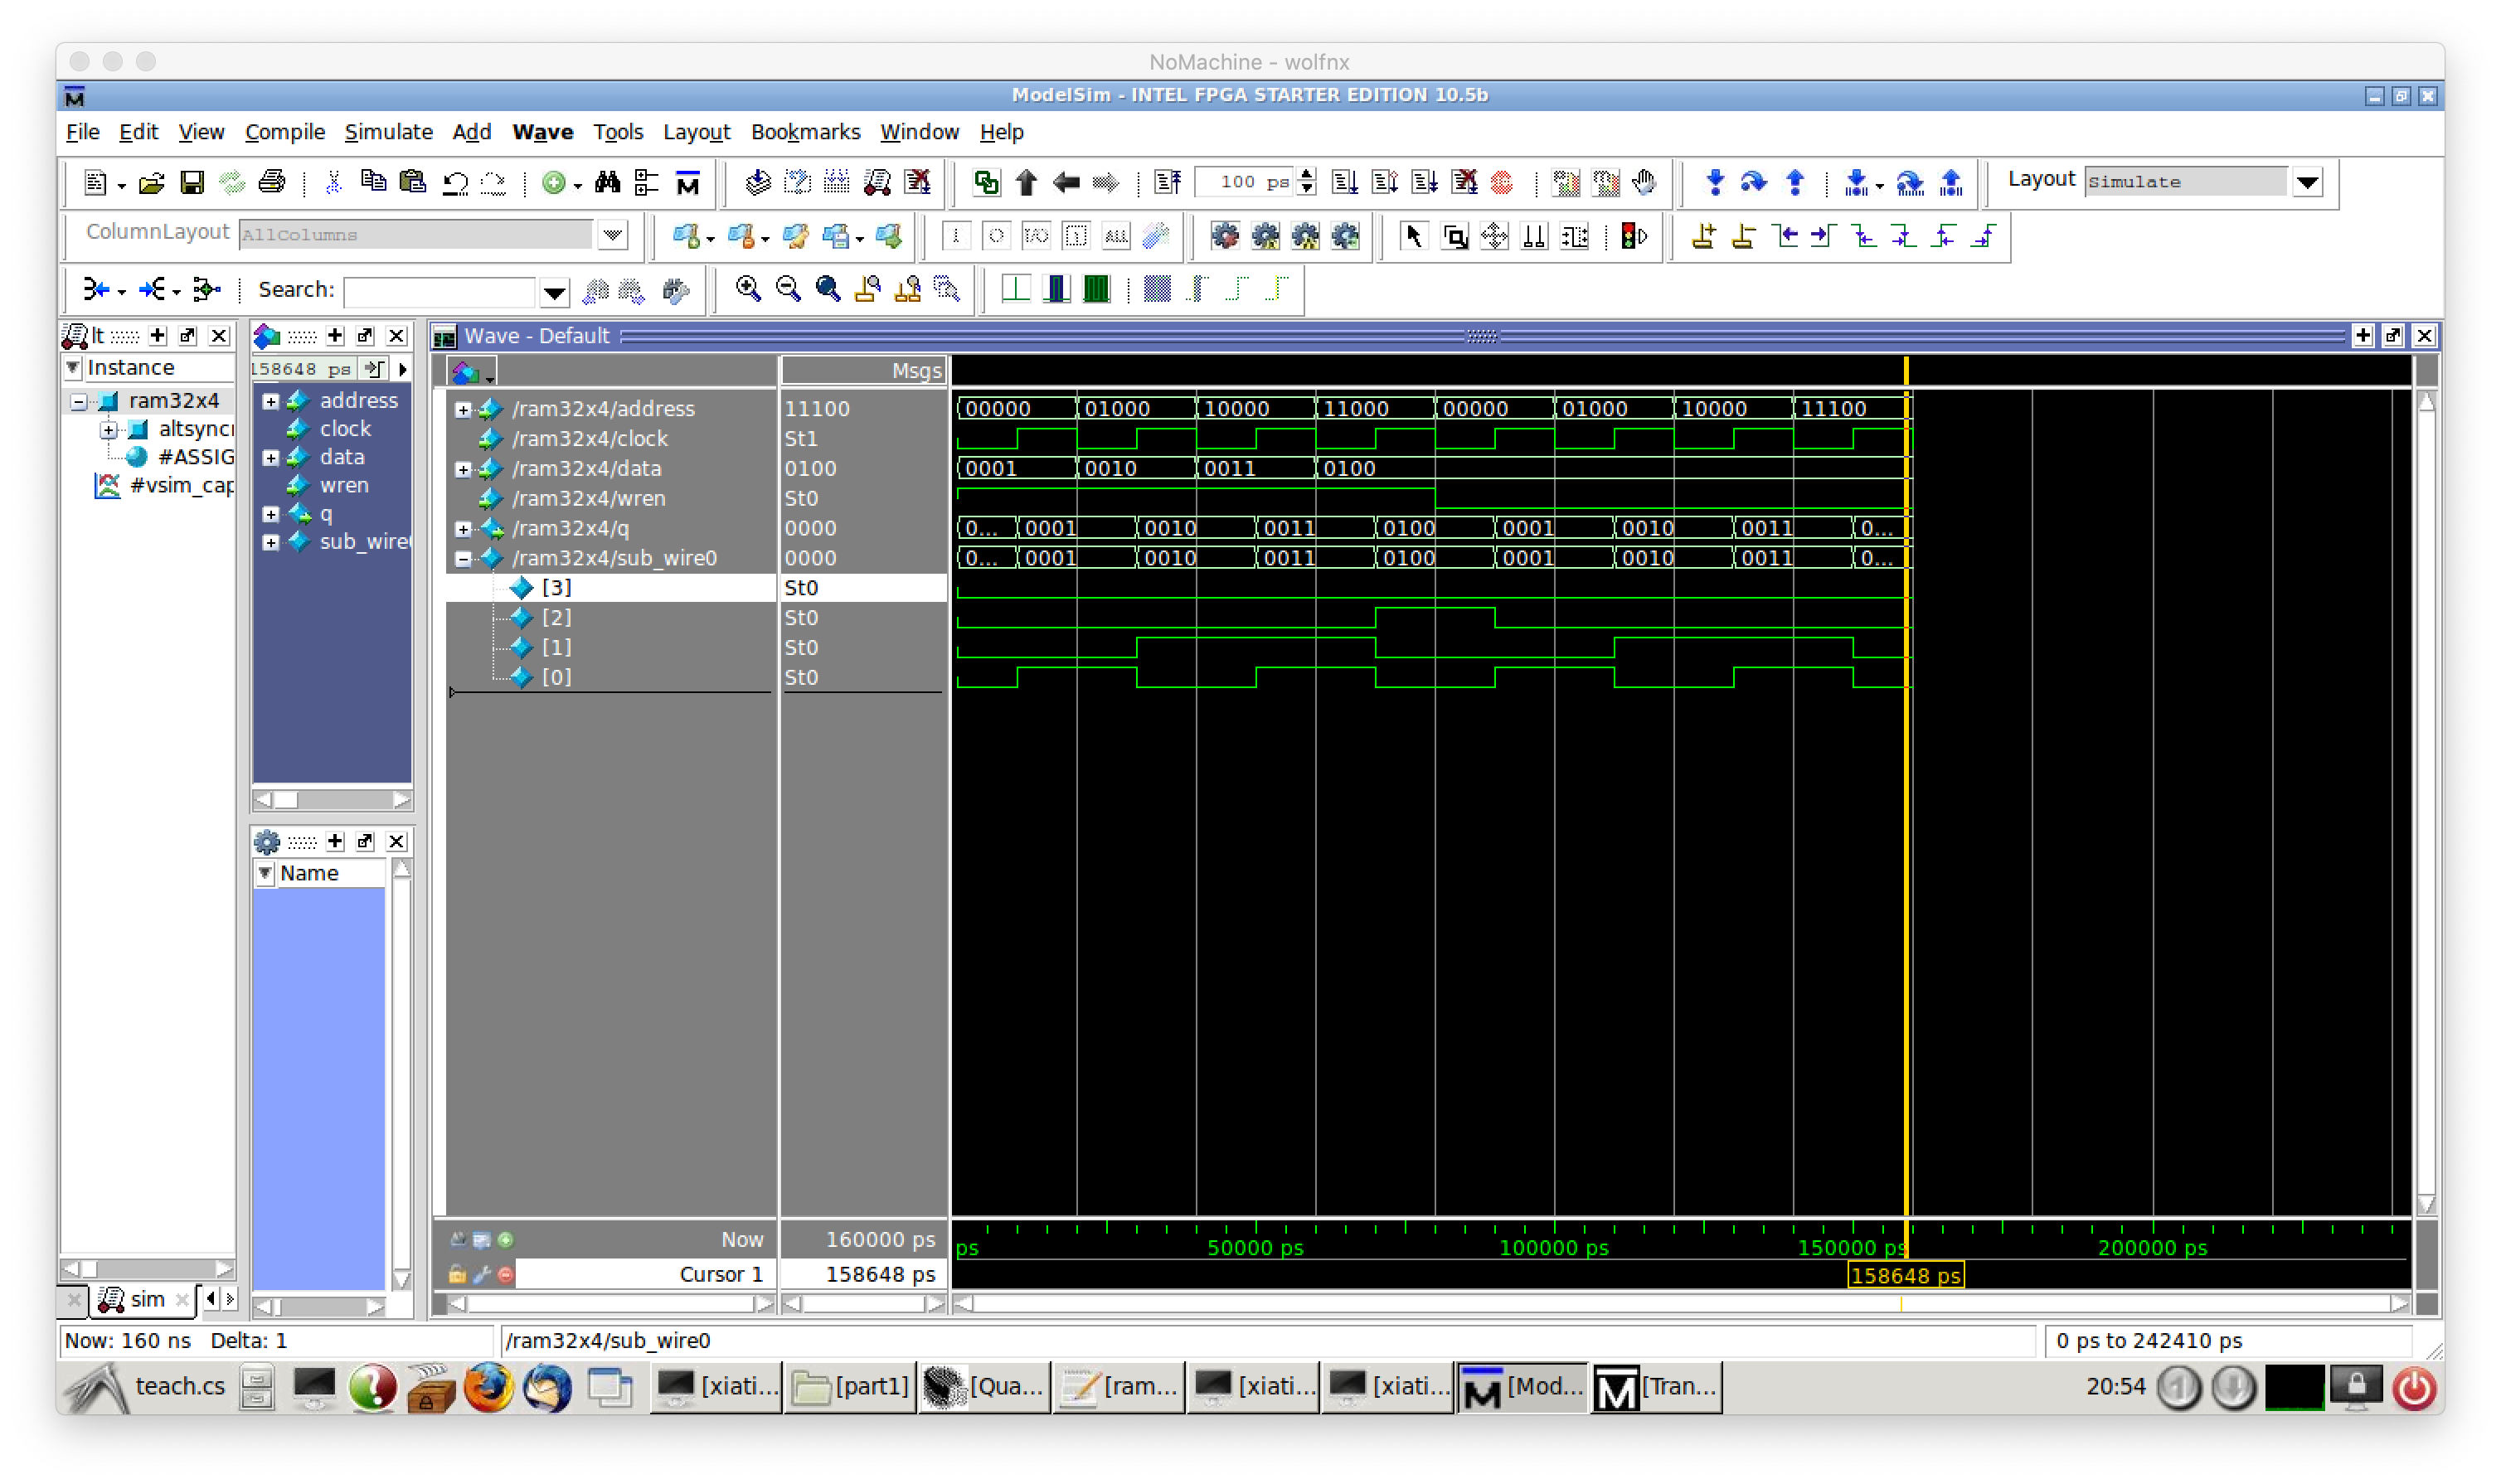
\includegraphics[scale=0.33]{part1_sim_ram32x4.png}
\end{center}

\paragraph{(10)} Here is my code that instantiates the \texttt{ram32x4.v} module from top level. Notice that this will only work if the \texttt{ram32x4.v} was included as part of the project. Here is my code

\begin{minted}{verilog}
    // SW[3:0] for data inputs
    // SW[8:4] for address inputs
    // SW[9] is write enable
    // KEY[0] clock
    
    // show address on HEX5 and HEX4
    // input data on HEX2
    // output data on HEX0 (output of memory)
    
    module ram_toplv(
            input [9:0] SW,
            input [0:0] KEY, 
            output [6:0] HEX5, 
            output [6:0] HEX4, 
            output [6:0] HEX2,
            output [6:0] HEX0
    );
        wire [3:0] ramout;
        
        ram32x4 ram_block(
            .address(SW[8:4]),
            .clock(KEY[0]),
            .data(SW[3:0]),
            .wren(SW[9]),
            .q(ramout[3:0])
        );
        
        // The last bit, for hex5
        hex_decoder hex5({3'b000, SW[8]}, HEX5[6:0]);
        hex_decoder hex4(SW[7:4], HEX4[6:0]);
        hex_decoder hex2(SW[3:0], HEX2[6:0]);
        hex_decoder hex0(ramout[3:0], HEX0[6:0]);
    
    endmodule
    
    // borrowed from lab6 starter code
    module hex_decoder(hex_digit, segments);
        input [3:0] hex_digit;
        output reg [6:0] segments;
    
        always @(*)
            case (hex_digit)
                4'h0: segments = 7'b100_0000;
                4'h1: segments = 7'b111_1001;
                4'h2: segments = 7'b010_0100;
                4'h3: segments = 7'b011_0000;
                4'h4: segments = 7'b001_1001;
                4'h5: segments = 7'b001_0010;
                4'h6: segments = 7'b000_0010;
                4'h7: segments = 7'b111_1000;
                4'h8: segments = 7'b000_0000;
                4'h9: segments = 7'b001_1000;
                4'hA: segments = 7'b000_1000;
                4'hB: segments = 7'b000_0011;
                4'hC: segments = 7'b100_0110;
                4'hD: segments = 7'b010_0001;
                4'hE: segments = 7'b000_0110;
                4'hF: segments = 7'b000_1110;
                default: segments = 7'h7f;
            endcase
    endmodule    
\end{minted}

\paragraph{(11)} Here is the schematic for the design
\begin{center}
    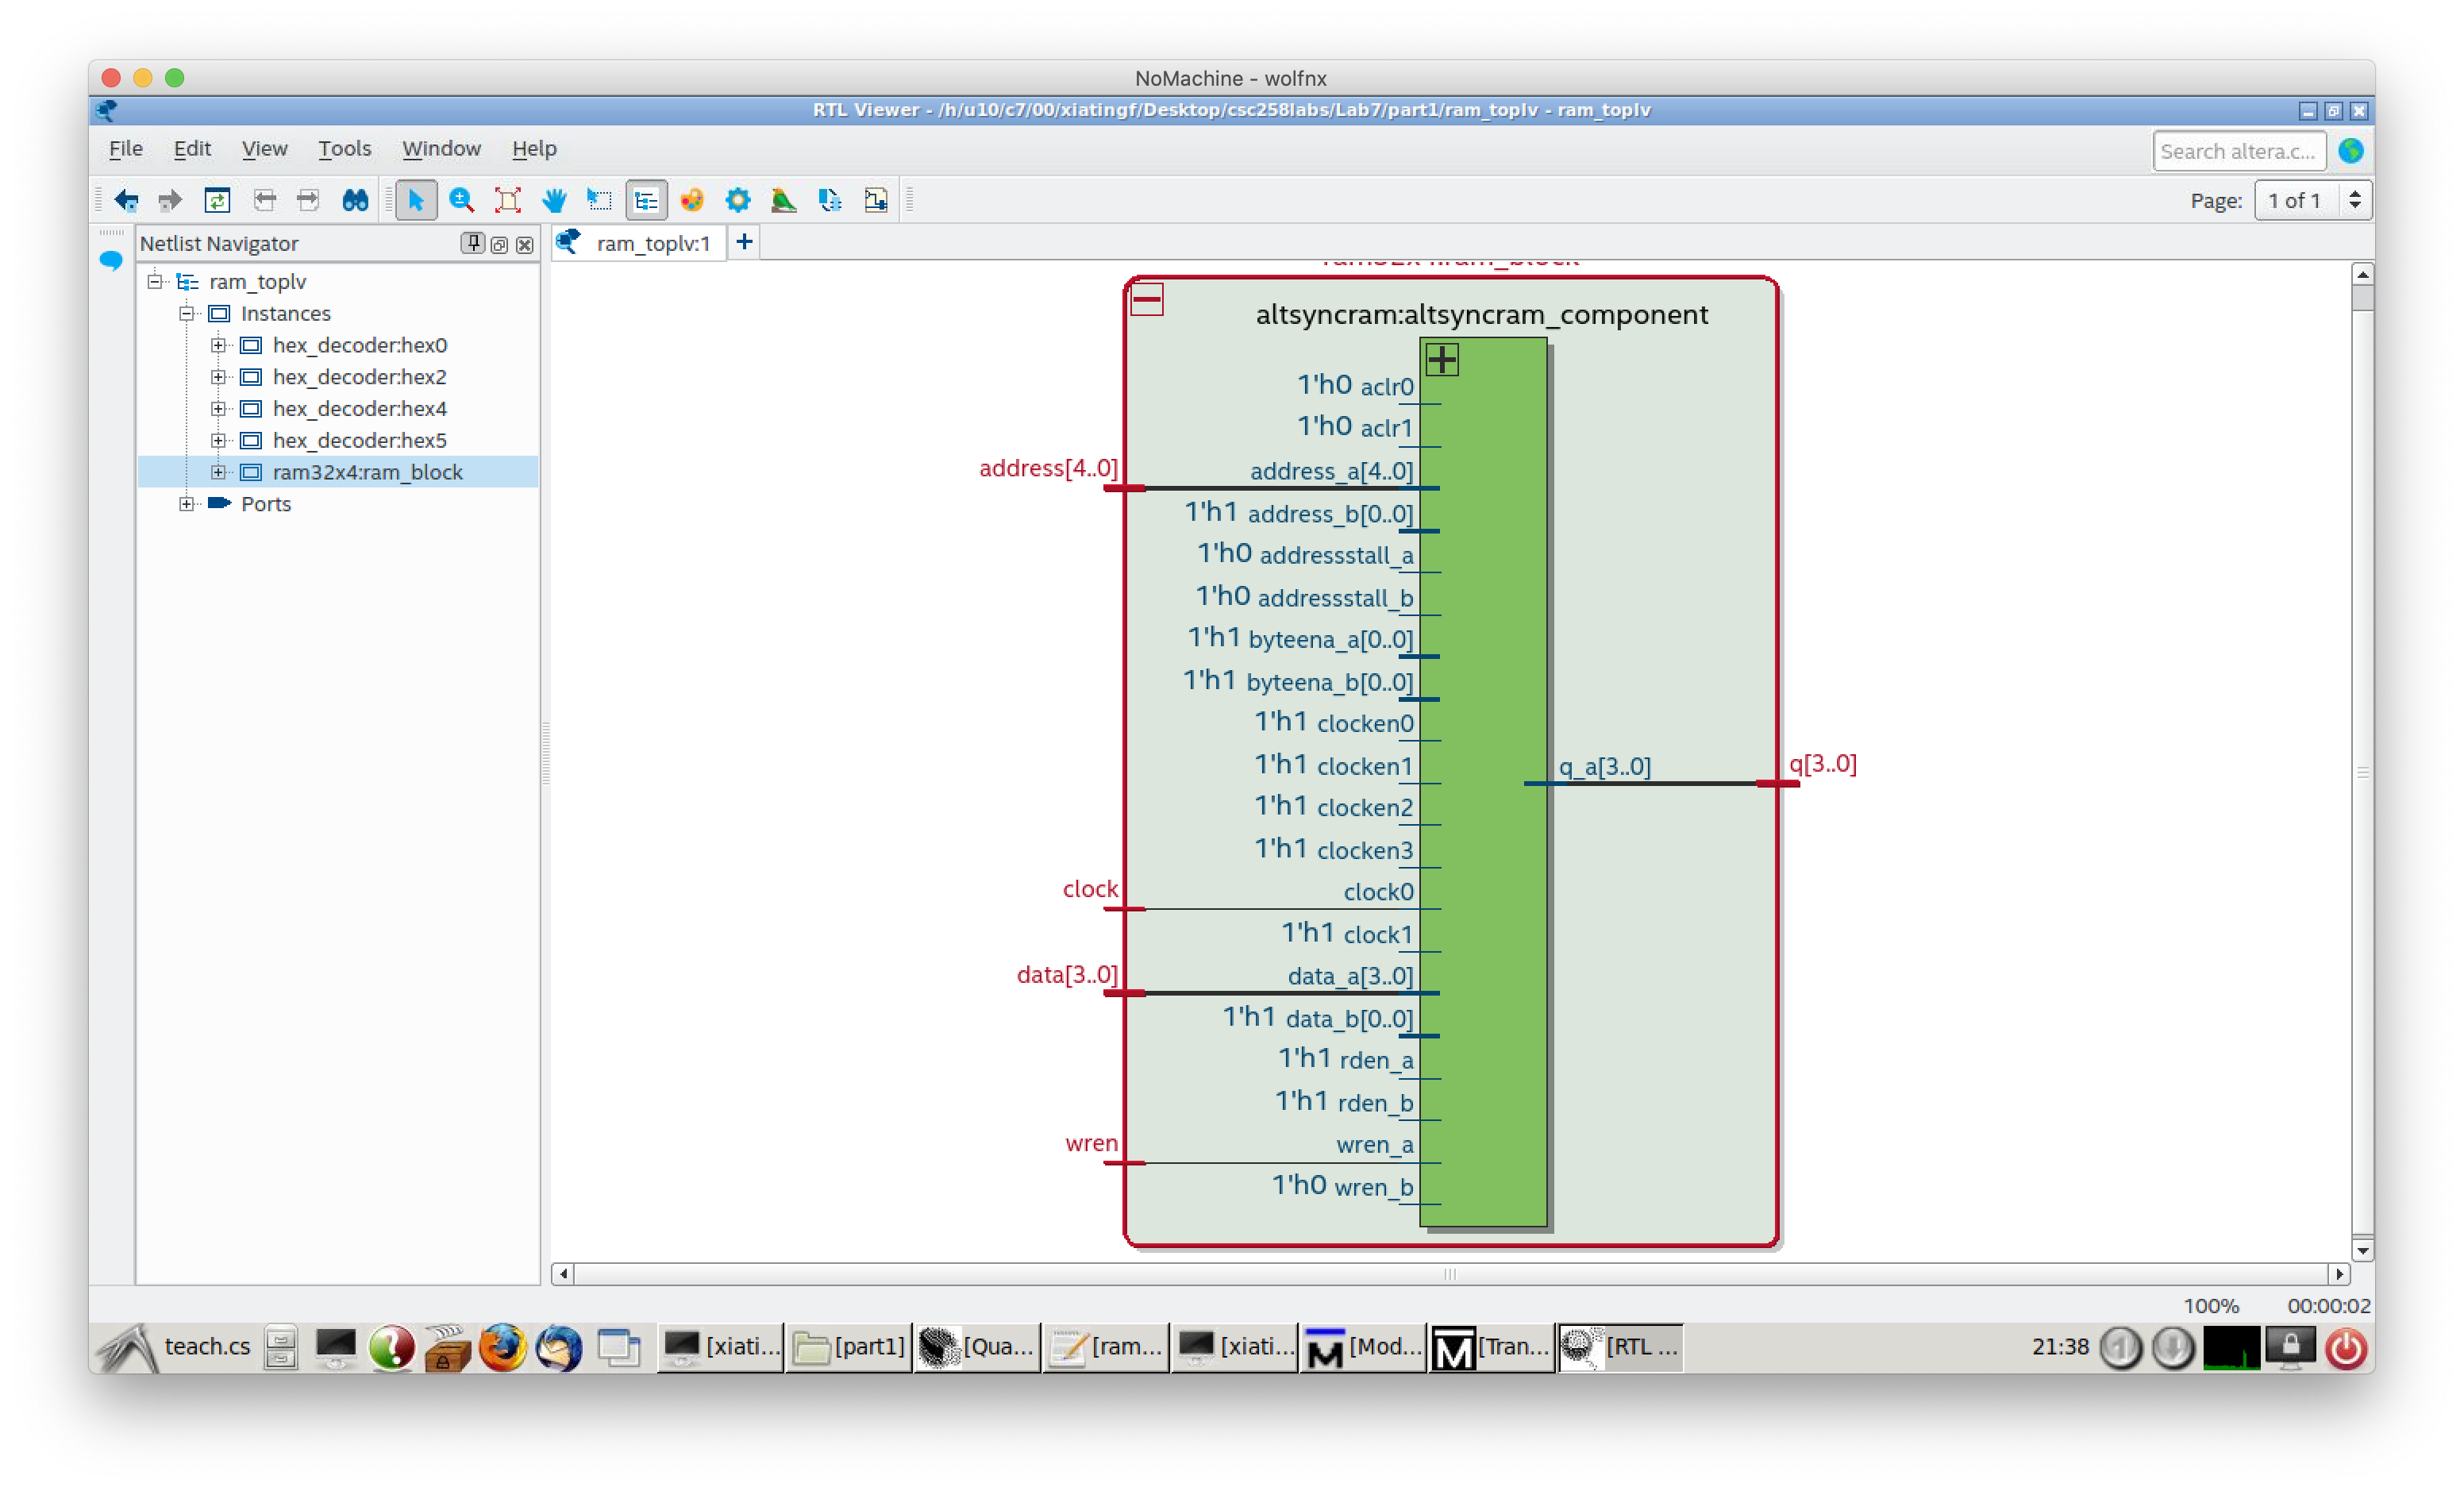
\includegraphics[scale=0.32]{part1_memory_block.png}
    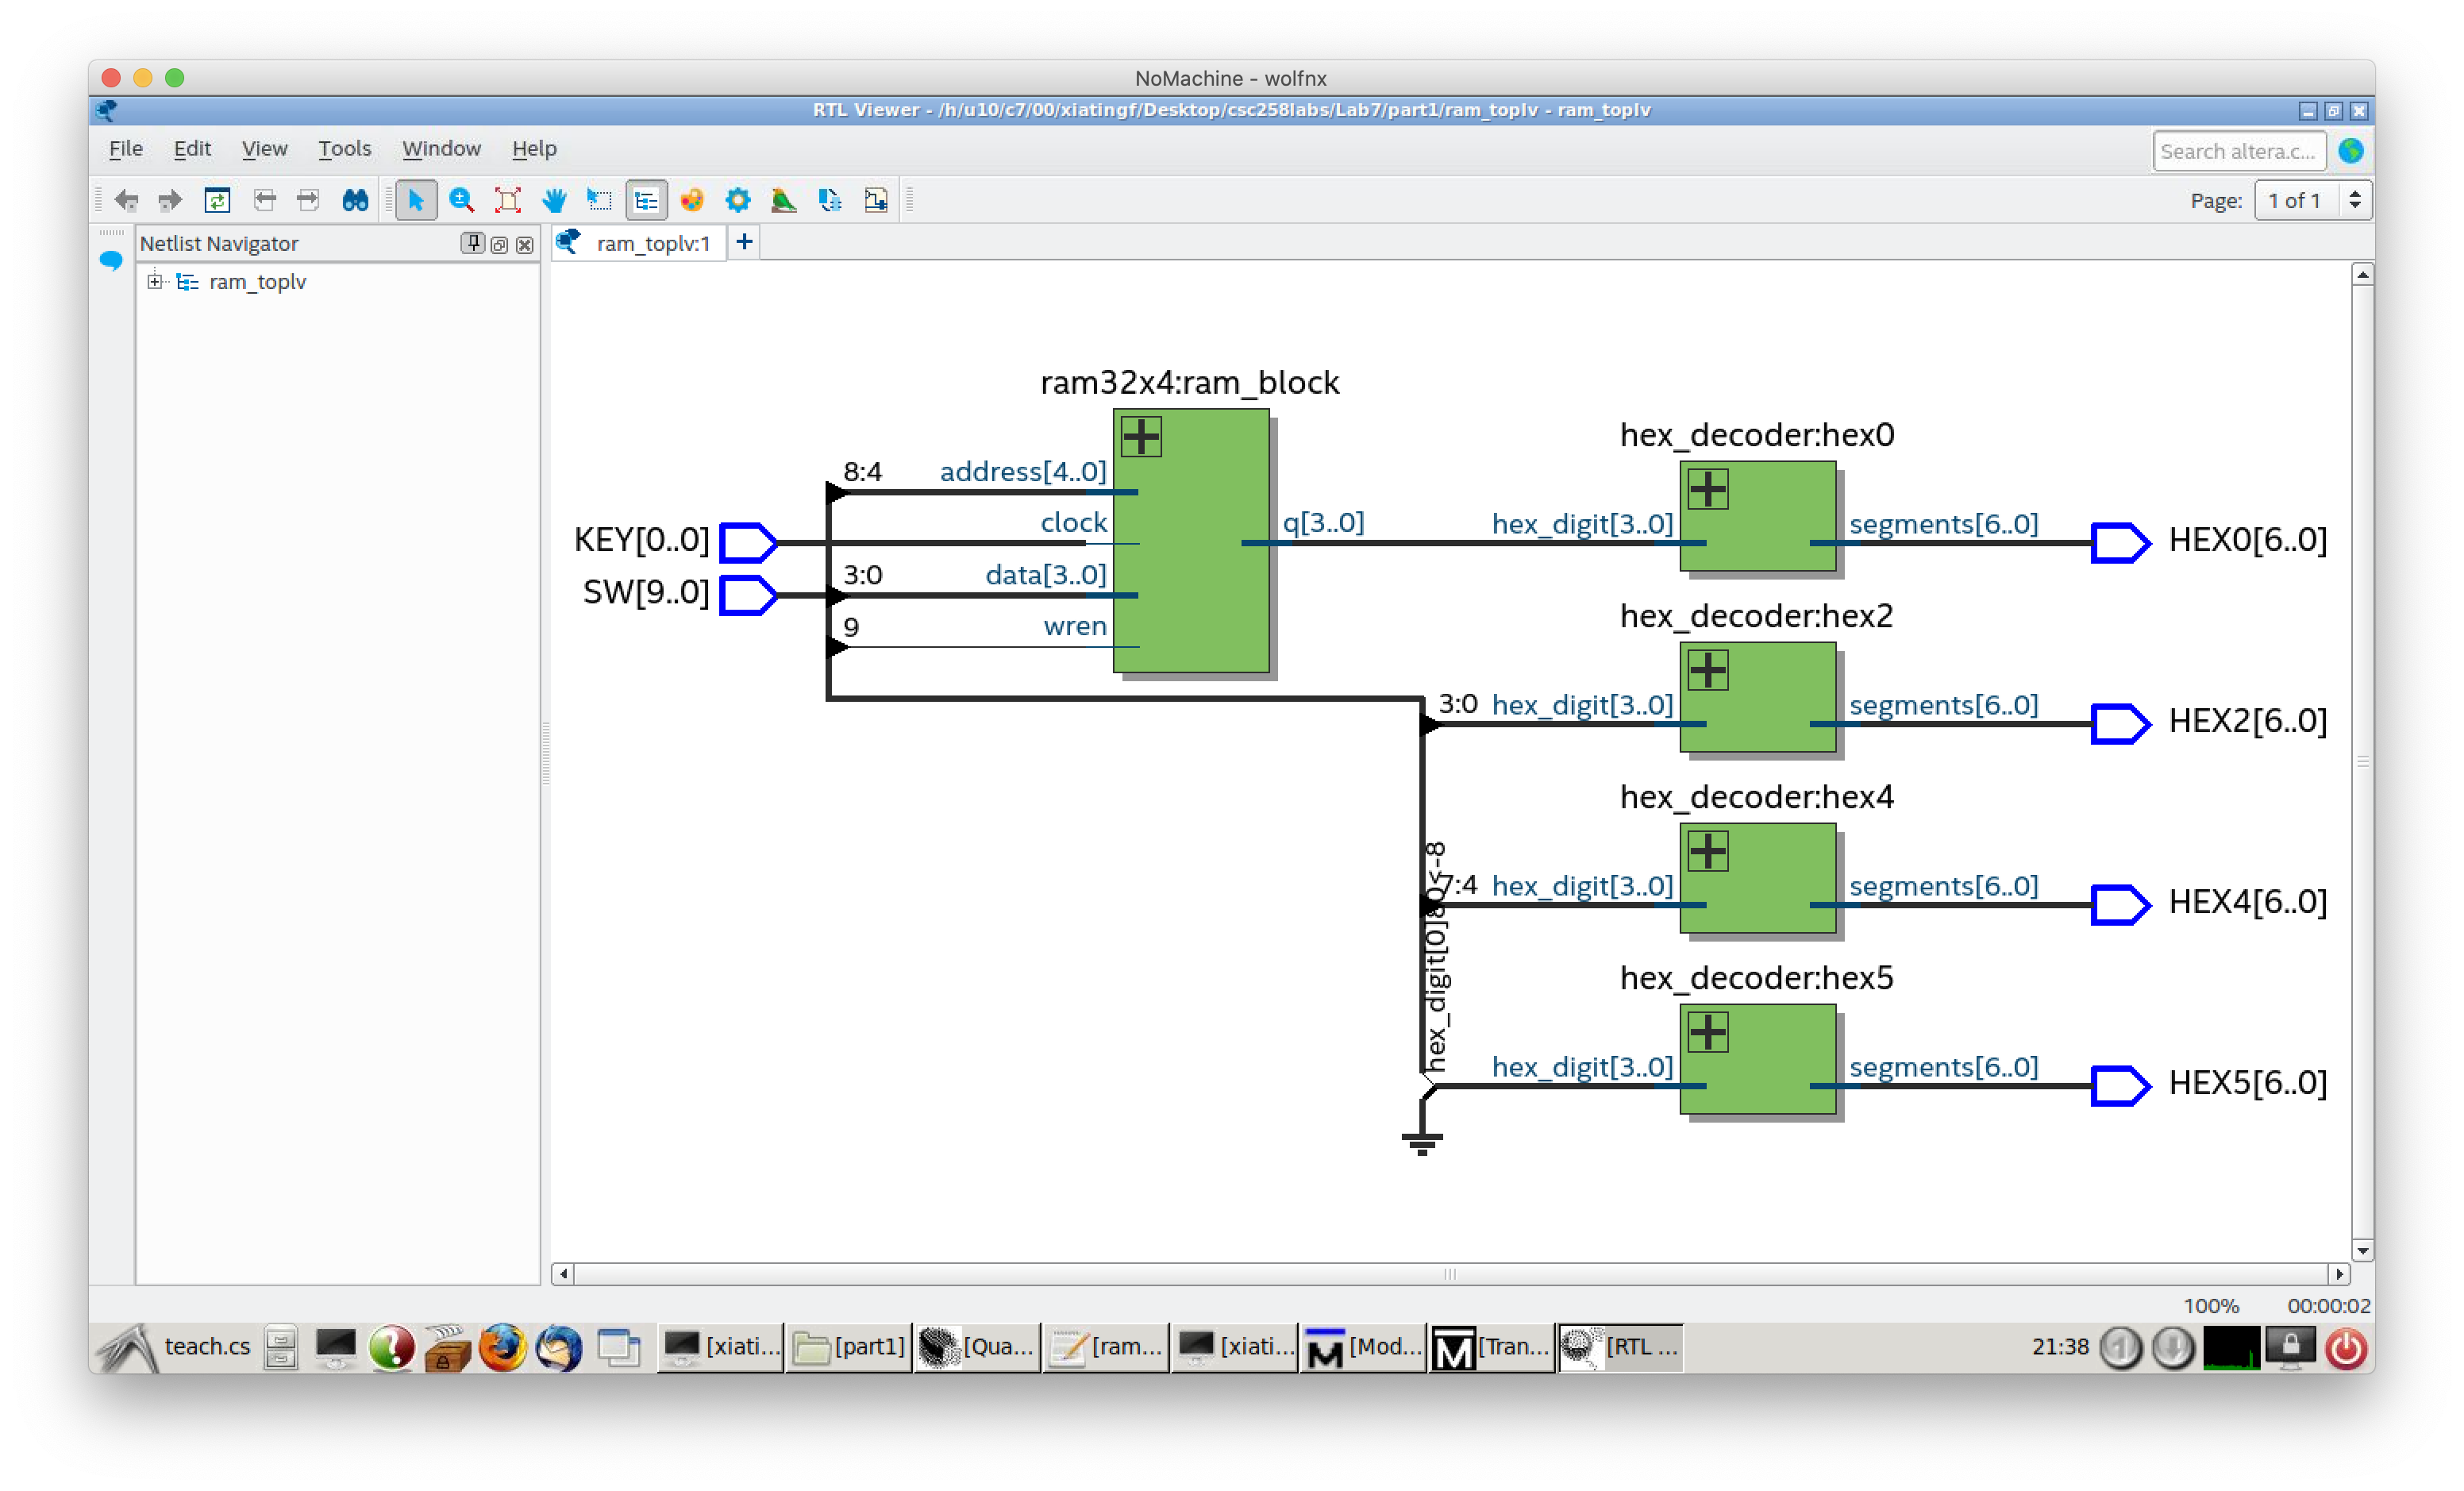
\includegraphics[scale=0.32]{part1_total_design.png}
\end{center}

\section*{PART II}



\end{document}
